% !Mode:: "TeX::UTF-8"
\documentclass{svk_long_sk}

\begin{document}
\title{ViDA: Vizualizácia distribuovaných algoritmov}

\author{Michal Anderle\inst{1}
\email{zaba@ksp.sk}
\and 
Ján Hozza\inst{1}
\email{janoh@ksp.sk}}

\supervisor{Jakub Kováč\inst{2}
\email{kuko@ksp.sk}}

%% nasleduje kratka verzia nazvu clanku a 
%% zoznam autorov (bez krstnych mien)
%% tieto informacie sa zobrazuju v hlavicke
\titlerunning{ViDA}
\authorrunning{Hozza and Anderle}

\institute{
Katedra informatiky,
FMFI UK,
Mlynská Dolina
842~48~Bratislava
\and
Katedra informatiky,
FMFI UK,
Mlynská Dolina
842~48~Bratislava}

\maketitle

\import abstract

\import uvod
\section{Úvod a príklady}

Tento článok používa \LaTeX\ štýl {\tt svk\_long\_sk.cls}.
\emph{Nemeňte tento štýl, veci súvisiace s fontami,
veľkosťou stránky, číslovaním strán a podobne.}

\subsection{Ukážkový text}
Nech $S=[s_{ij}]$ ($1\leq i,j\leq n$) je $(0,1,-1)$-matica
veľkosti $n$. Potom $S$ je {\em znamienkovo-nesingulárna matica}
(SNS-matrix), ak každá reálna matica so znamienkovým vzorom
matice $S$ je nesingulárna. V súčasnosti bol silný záujem
o konštrukciu a charakterizáciu
SNS-matíc \cite{bs}, \cite{klm}. Záujem bol tiež o štúdium silných foriem
znamienkovej nesingularity \cite{djd}. V tomto článku ponúkame
nové zovšeobecnenie SNS-matíc a skúmame niektoré ich základné vlastnosti.
 
\subsection{Číslovaný zoznam}
V tomto článku sa zaoberáme výpočtom integrálov nasledujúcich druhov:
\begin{equation}
\int_a^b \left( \sum_i E_i B_{i,k,x}(t) \right)
         \left( \sum_j F_j B_{j,l,y}(t) \right) dt,\label{problem}
\end{equation}
\begin{equation}
\int_a^b f(t) \left( \sum_i E_i B_{i,k,x}(t) \right) dt,\label{problem2}
\end{equation}
kde $B_{i,k,x}$ je $i$-ty B-splajn stupňa $k$ definovaný v uzloch
$x_i, x_{i+1}, \ldots, x_{i+k}$.
Budeme predpokladať, že B-splajny sú normalizované tak, že ich integrál je 
jednotkový.
Splajny môžu byť rôznych stupňov a môžu byť definované v navzájom rôznych 
postupnostiach uzlov
$x$ and $y$.
Limity integrácie budú často
od $-\infty$ po
$+\infty$. Všimnite si, že (\ref{problem}) je špeciálnym prípadom
(\ref{problem2}),
kde $f(t)$ je splajn.

Budeme predpokladať:
\begin{enumerate}
\item Toto.
\item Hento.
\item Tamto.
\end{enumerate}

\subsection{Matematické rovnice (equations and \{{\tt eqnarray}\}s)}

Napríklad,
\begin{equation}
\langle (A_{1},B_{1}), (A_{2},B_{2})\rangle := \langle A_{1},A_{2}\rangle 
+ \langle B_{1},B_{2}\rangle,\label{eq2.10}
\end{equation}

je rovnica. Podobne,

\begin{eqnarray}
 F'(U,V)(H,K) &=& \langle R(U,V),H\Sigma V^{T} + U\Sigma K^{T}\nonumber\\
             && - P(H\Sigma V^{T} + U\Sigma K^{T})\rangle \nonumber \\
         &=& \langle R(U,V),H\Sigma V^{T} + U\Sigma K^{T}\rangle\nonumber \\
&=& \langle R(U,V)V\Sigma^{T},H\rangle + \nonumber\\
  &&    \langle \Sigma^{T}U^{T}R(U,V),K^{T}\rangle.    \label{eq2.11}
\end{eqnarray}

Taktiež
\begin{eqnarray}
 \nabla F(U,V) &=& (R(U,V)V\Sigma^{T},R(U,V)^{T}U\Sigma )\nonumber\\
 && \in R^{m \times m} \times R^{n \times n}.   \label{eq2.12}
\end{eqnarray}

Aj
\begin{equation}
\frac{d(U,V)}{dt} = -g(U,V) 	\label{eq2.15}
\end{equation}
je rovnica.

\subsection{Lorem ipsum}

Lorem ipsum dolor sit amet, consectetur adipisicing elit, sed do eiusmod tempor incididunt ut labore et dolore magna aliqua. Ut enim ad minim veniam, quis nostrud exercitation ullamco laboris nisi ut aliquip ex ea commodo consequat. Duis aute irure dolor in reprehenderit in voluptate velit esse cillum dolore eu fugiat nulla pariatur. Excepteur sint occaecat cupidatat non proident, sunt in culpa qui officia deserunt mollit anim id est laborum.
 
\section{Hlavné výsledky} 
 
\begin{theorem} 
\label{th:prop} 
Dvojica matíc $(S,C)$ je {\rm SNS}-maticový pár, ak všetky nenulové
koeficienty jeho charakteristického polynómu majú rovnaké znamienko a
ak aspoň jeden z koeficientov je nenulový.
\end{theorem} 
 
\begin{proof}
Je to naozaj tak. \qquad\end{proof} 
 
\begin{lemma}[{\rm Stabilita}]
\label{stability}
Stabilita je fajn, ak
\begin{equation}
\label{Gron}
\frac {d}{dt} \| \epsilon (t) \| _{1,2}  \leq B
   ( h^{q-3/2} + \| \epsilon (t) \|_{1,2})\;.
\end{equation}
\end{lemma}

\subsection{Lorem ipsum}

Lorem ipsum dolor sit amet, consectetur adipisicing elit, sed do eiusmod tempor incididunt ut labore et dolore magna aliqua. Ut enim ad minim veniam, quis nostrud exercitation ullamco laboris nisi ut aliquip ex ea commodo consequat. Duis aute irure dolor in reprehenderit in voluptate velit esse cillum dolore eu fugiat nulla pariatur. Excepteur sint occaecat cupidatat non proident, sunt in culpa qui officia deserunt mollit anim id est laborum.

\subsection{Experimenty}
Hrali sme sa s
\begin{eqnarray} 
{\displaystyle \Delta w + c e^w + d{ {\partial w}\over{\partial x} } } 
&=&{\displaystyle f \quad {\rm v}\ D, }\nonumber\\[-1.5ex]
\label{bratu} \\[-1.5ex]
{\displaystyle w }&=&{\displaystyle 0 \quad {\rm na}\ \partial D , } \nonumber
\end{eqnarray} 
kde $c$ a $d$ sa nemenia. Aj \cite{Brown-Saad1} to robili.

Dopadlo to tak, ako ukazuje Obr.~\ref{diff} a Tab.~\ref{diffstats}.

\begin{figure}
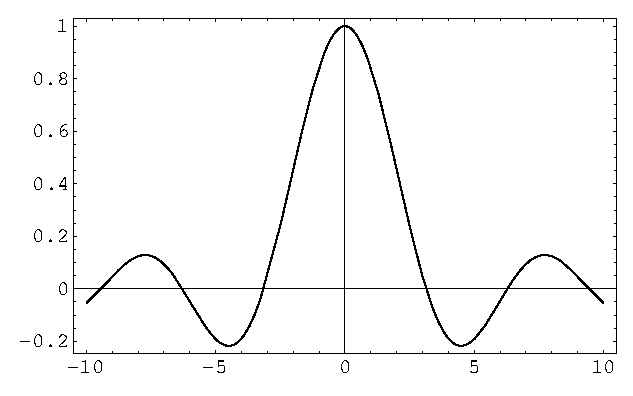
\includegraphics[width=\columnwidth]{fig}
\caption{Graf funkcie $\sin(x)/x$.} 
\label{diff} 
\end{figure}  
%% ak je vas obrazok siroky a chcete ho zobrazit
%% cez dva stlpce, pouzite \begin{figure*}...\end{figure*}
 
\begin{table*}
\caption{Táto tabuľka obsahuje rôzne dáta namerané pri kadejakých
experimentoch.}

\begin{center} \footnotesize
\begin{tabular}{|c|c|c|c|c|c|} \hline  
&& Počet & Počet & Čas & Štandardná \\ 
Metóda & $\epsilon$ & Iterácie & Iný čas (Seconds) & Odchýlka \\ \hline 
\lower.3ex\hbox{EHA2} & \lower.3ex\hbox{$10^{-10}$} & \lower.3ex\hbox{26} &  
\lower.3ex\hbox{32} & \lower.3ex\hbox{47.12} & \lower.3ex\hbox{.1048} \\ 
FD2 & $10^{-10}$ & 26 & 58 & 53.79 & .1829 \\ \hline  
\lower.3ex\hbox{EHA4} & \lower.3ex\hbox{$10^{-12}$} & \lower.3ex\hbox{30} &  
\lower.3ex\hbox{42} & \lower.3ex\hbox{56.76} & \lower.3ex\hbox{.1855} \\  
FD4 & $10^{-12}$ & 30 & 132 & 81.35 & .3730 \\ \hline  
\lower.3ex\hbox{EHA6} & \lower.3ex\hbox{$10^{-12}$} & \lower.3ex\hbox{30} &  
\lower.3ex\hbox{48} & \lower.3ex\hbox{58.56} & \lower.3ex\hbox{.1952} \\ 
FD6 & $10^{-12}$ & 30 & 198 & 100.6 & .3278 \\ \hline  
\end{tabular}
\end{center} 
\label{diffstats} 
\end{table*}
%% ak je vasa tabulka uzka a chcete, aby zaberala iba
%% jeden stlpec, pouzite \begin{tabular}...\end{tabular}

\section*{Poďakovanie}
Ďakujeme FMFI UK za podporu.

\nocite{*}
\bibliographystyle{apalike}
\bibliography{references}

%% citacie ulozte do suboru references.bib
%% na populaciu zoznamu literatury pouzite program
%%
%% bibtex references
%%
%% po ktorom je potrebne dokument znova zlatexovat

\end{document}

